\section{Grundlagen}
\label{sec:grundlagen}
In diesem Versuch werden verschiedene Schaltungen mit Hilfe des
Operationsverstärkers realisiert.
Zunächst wird auf die physikalischen Eigenschaften eingegangen,
woraufhin verschiedene Schaltungen skizziert und schließlich
realisiert werden.

\subsection{Eigenschaften des Operationsverstärkers}
\label{subsec:eigenschaften}
Die wichtigste elektrische Eigenschaft des Operationsverstärkers
ist die Proportionalität der Ausgangsspannung $U_\text{A}$ zur
Differenz der Eingangsspannungen $U_\text{p}$ und $U_\text{N}$:
\begin{equation}
\label{eq:proportionalität}
    U_\text{A} = V(U_\text{p} - U_\text{N})\,,
\end{equation}
wobei $V$ die Leerlaufverstärkung bezeichnet.
Diese Beziehung gilt in einem Spannungsbereich
$-U_\text{B} < U_\text{A} < U_\text{B}$, der durch die Betriebsspannung
$U_\text{B}$ bestimmt ist. Ausserhalb dieses Bereichs läuft die
Ausgangsspannung in eine Sättigung.
Die Eingangsspannung $U_\text{p}$ wird nicht invertiert, während die Spannung
$U_\text{N}$ invertiert wird -- der Verstärker besitzt also einen
nicht-invertierenden und einen invertierenden Eingang.

Aus technischer Sicht entspricht der Operationsverstärker einem
gleichstromgekoppeltem Differenzverstärker. Er ist in Abbildung
\ref{fig:op} dargestellt.
\begin{figure}
    \centering
    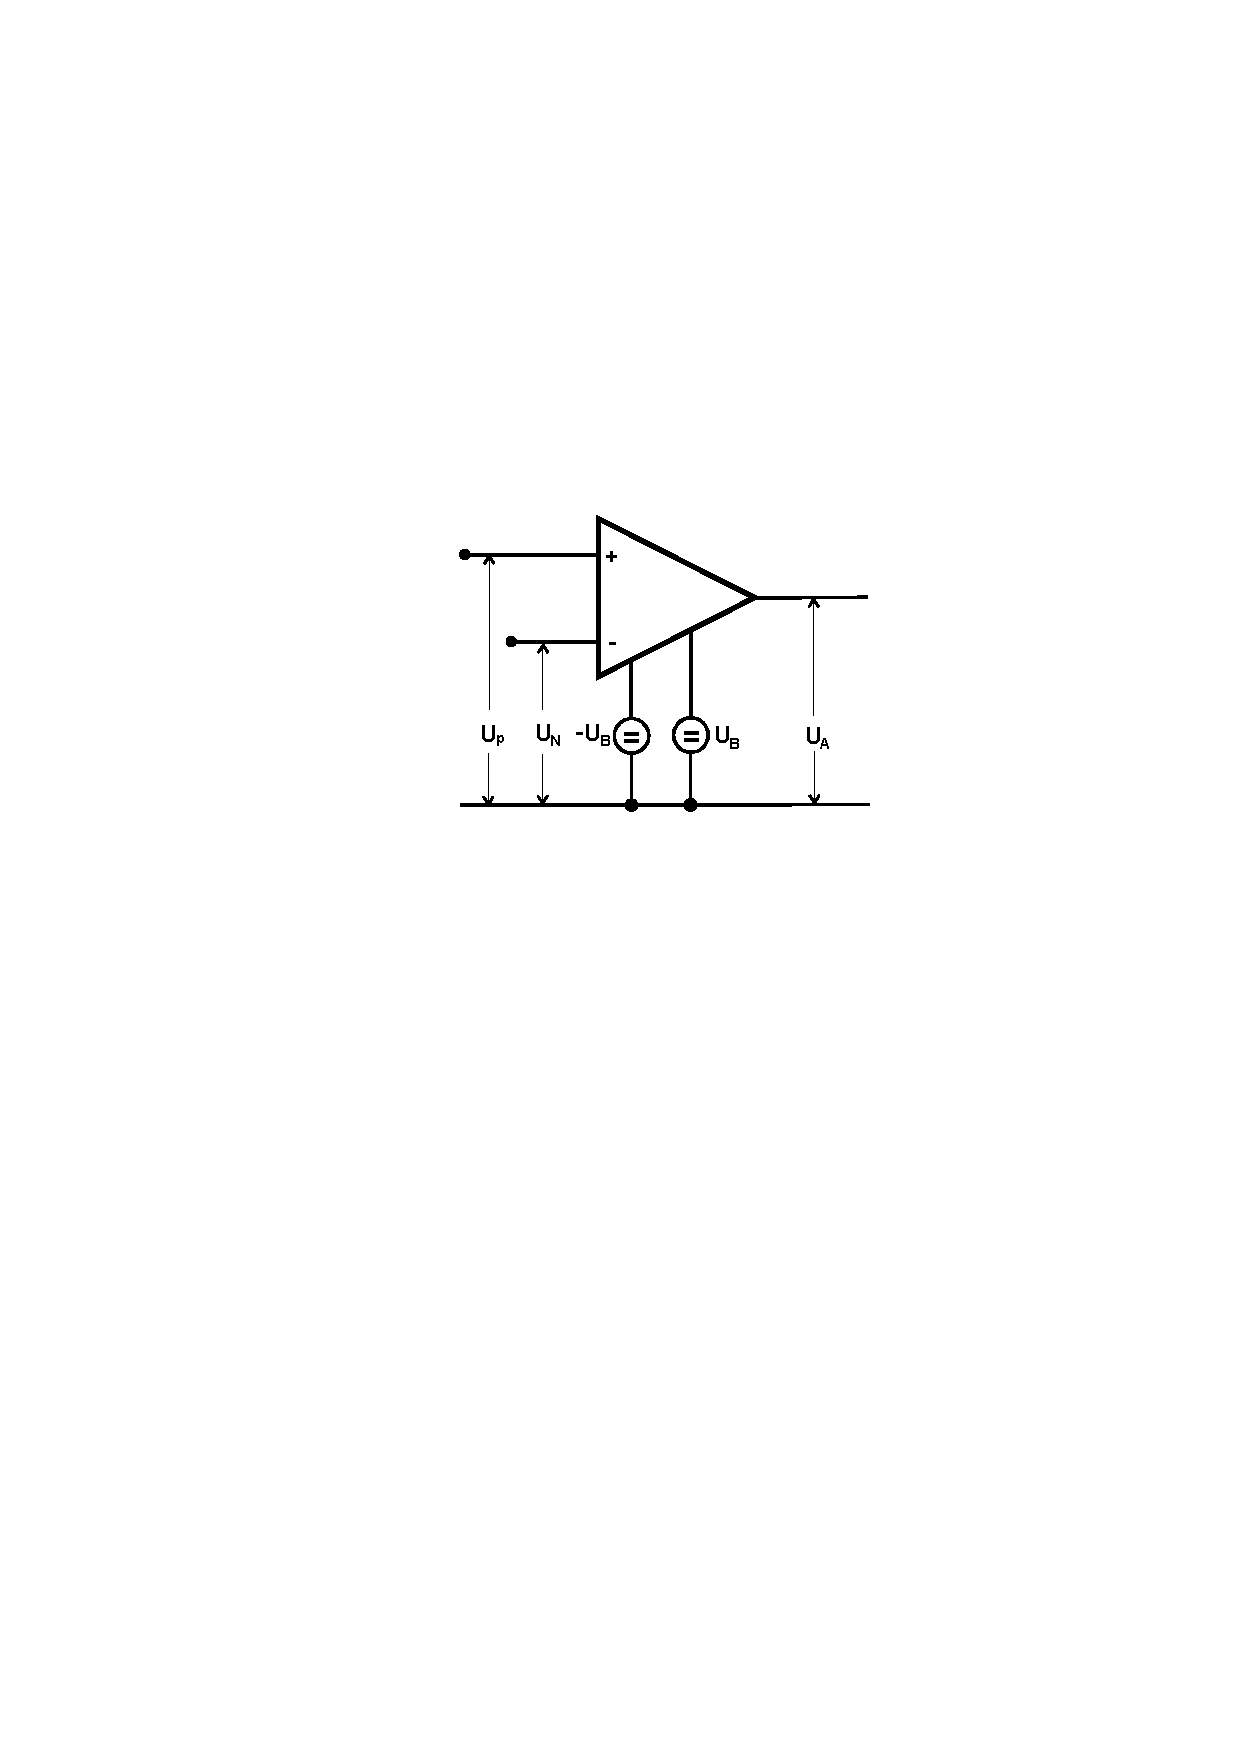
\includegraphics[width=0.7\linewidth]{img/op.pdf}
    \caption{
        Schaltbild eines Operationsverstärkers mit Ausgangsspannung
        $U_\text{A}$ und Eingangsspannungen $U_\text{p}$ und
        $U_\text{N}$ \cite{V51}.
    }
    \label{fig:op}
\end{figure}
Neben der meist frequenzabhängigen Leerlaufverstärkung $V$ besitzt der
Operationsverstärker weitere Kenngrößen, wie die Eingangswiderstände,
$r_\text{e,p}$ und $r_\text{e,N}$, sowie 
einen Ausgangswiderstand $r_\text{a}$.
Um Rechnungen zu Vereinfachen gilt für einen idealen Operationsverstärker
\begin{equation}
\label{eq:id-verstärker}
    V = \infty\,,\qquad r_\text{e} = \infty\,,\qquad r_\text{a} = 0\,.
\end{equation}

Im Gegensatz dazu müssen zur theoretischen Beschreibung eines realen
Operationsverstärkers zusätzliche Kenngrößen in Betracht gezogen werden.

Die Gleichtaktverstärkung
\begin{equation}
\label{eq:gleichtaktverstärkung}
    V_\text{Gl} = \frac{\Delta U_\text{A}}{\Delta U_\text{Gl}}
\end{equation}
berücksichtigt geringe Asymmetrien der beiden Vertärkungskanäle.
Dabei bezeichnen $\Delta U_\text{A}$ die Differenz der Ausgangsspannung zu
\num{0} und $\Delta U_\text{Gl}$ den Unterschied der -- eigentlich gleichen --
Eingangsspannungen.

Die auf Grund endlicher Eingangswiderstände $r_\text{e}$ auftretenden
Eingangsströme werden mit $I_\text{p}$ und $I_\text{N}$ bezeichnet.
